\documentclass[11pt,a4j,fleqn]{jarticle}
\usepackage{amsmath,amsthm,amssymb}
\usepackage[dvipdfmx]{graphicx}

\title{包絡線定理レポート}
\author{大野 嵩侃}
\date{2014年6月7日}


\begin{document}

\maketitle

\section{はじめに}



\section{包絡線定理}

$x$をパラメタとする(微分可能な)関数$f(a,x)$について,$x$をある値$x_1$に固定すれば,$b=f(a,x_1)$を満たすような$a$と$b$の関係を表す曲線が1つ定まる.同様に、$x$を$x_2$に固定すれば,$b=f(a,x_2)$を満たすような$a$と$b$の関係を表す曲線がやはり1つ定まる.このように、$x$の値を変化させることで異なる曲線が定められるので,$b=f(a,x)$は$x$をパラメタとする$a-b$平面上の曲線群を表していると考えられる.$x$を連続的に変化させると,この曲線の形も連続的に変化する。\\
ここで、ある曲線$b=g(a)$が$b=f(a,x)$で表されるすべての曲線と接していて、かつ接点の軌跡となっているとき,$g(x)$を$f(a,x)$の包絡線という.
簡単な関数を用いて具体的に考えてみよう。\\
\begin{equation}
f(a, x) = x a - x^2\label{eq:1}
\end{equation}
とする。
\eqref{eq:1}式の右辺を平方完成すると
\begin{equation}
f(a,  x) = -\left(x - \frac{a}{2}\right)^2 + \frac{a^2}{4} \label{eq:2}
\end{equation}
と変形できる。
平方完成の式\eqref{eq:2}より, 
\begin{equation} 
\max_{x}f(a, x) = \frac{a^2}{4} \label{eq:3}
\end{equation}
よって, $x$にさまざまな値を代入して$a-b$グラフ上に描かれる複数の直線について, その包絡線$g(a)$は
\begin{equation} 
g(a) = \frac{a^2}{4} \label{eq:4}
\end{equation}
と表されることがわかる。\\

具体的に$x$の値をいくつかとって直線を重ねてみると, たしかに求めた$g(a)$に近い形が見えてくる。\\
たとえば$x$を$-2$から$2$まで$\displaystyle{\frac{1}{3}}$ずつ変化させて$13$本の直線を引いたものが図1\\
$x$を$-3$から$3$まで$\displaystyle{\frac{1}{5}}$ずつ変化させて$31$本の直線を引いたものが図2である。\\
\begin{figure}[p]
 \centering
 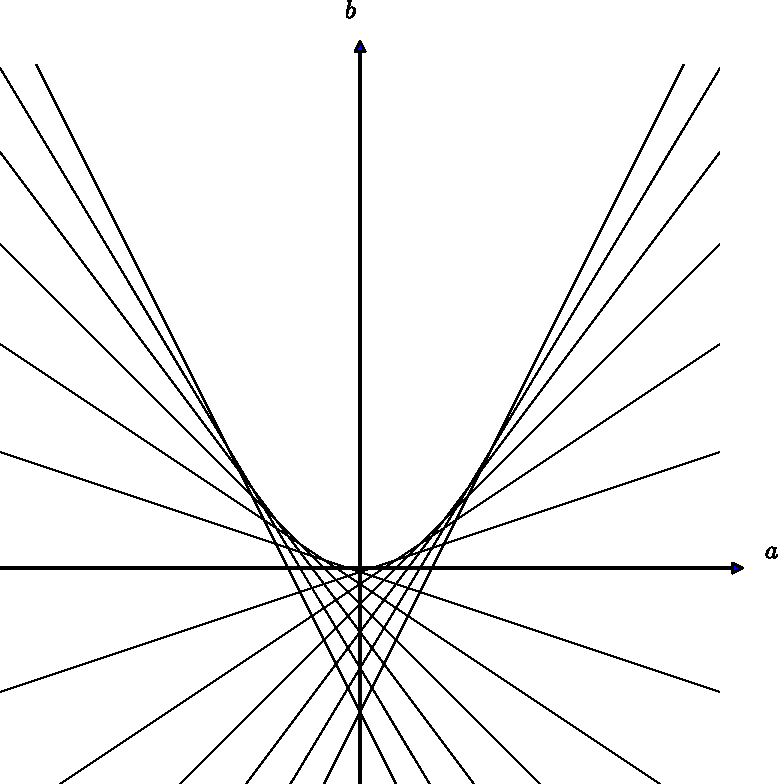
\includegraphics[scale=0.7]{envelope0.pdf}
 \caption{13本}
 \label{fig:1}
\end{figure}
\\
\begin{figure}[p]
 \centering
 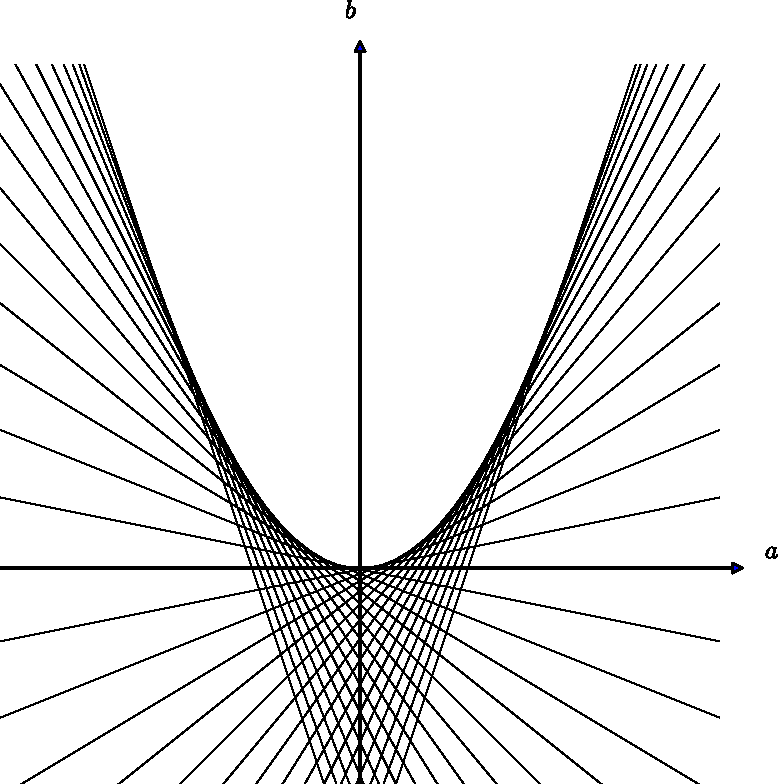
\includegraphics[scale=0.7]{envelope1.pdf}
 \caption{31本}
 \label{fig:2}
\end{figure}


引用の例:尾山・安田\cite{OyamaYasuda11}.


\subsection{サブセクションのタイトル}

必要ならサブセクションを作る.


\newpage
\section{Pythonプログラム}
\subsection{コード}
\begin{quote}
\begin{verbatim}
1  	from __future__ import division
2  	from numpy import linspace
3  	from numpy import fabs
4  	from numpy import array
5  	from mpl_toolkits.axes_grid.axislines import SubplotZero
6  	import matplotlib.pyplot as plt
7  	
8  	
9  	def f(x, a):
10 	    return a*x-x**2
11 	p = -3
12 	q = 3
13 	n = 12
14 	a_min = -10
15 	a_max = 10
16 	y_min = -6
17 	y_max = y_min+a_max-a_min
18 	plt.figtext(0.85, 0.35, '$a$')
19 	plt.figtext(0.5, 0.95, '$b$')
20 	fig = plt.figure(1)
21 	ax = SubplotZero(fig, 111)
22 	fig.add_subplot(ax)
23 	ax.axhline(linewidth=1.0, color="black")
24 	ax.axvline(linewidth=1.0, color="black")
25 	ax.set_xticks([])
26 	ax.set_yticks([])
27 	ax.set(aspect=1)
28 	for direction in ["xzero", "yzero"]:
29 	    ax.axis[direction].set_axisline_style("-|>")
30 	    ax.axis[direction].set_visible(True)
31 	for direction in ["left", "right", "bottom", "top"]:
32 	    ax.axis[direction].set_visible(False)
33 	plt.ylim(ymin=y_min)
34 	plt.ylim(ymax=y_max)
35 	a = array([a_min, a_max])
36 	for i in range(n):
37 	    r = p+(q-p)*i/(n-1)
38 	    b = f(r, a)
39 	    ax.plot(a, b, 'k', linewidth=0.5, alpha=1)'
40 	plt.show()
\end{verbatim}
\end{quote}

\subsection{コードの解説}
\begin{quote}
\begin{verbatim}
1~6行目では必要な機能を各モジュールからインポートした。
9~19行目にはこちらで入力する引数がまとめてある。詳細な情報は以下に記す。
9, 10行目ではf(x, a)を定義している。xに具体的な値が代入されることで、a-b平面上の直線、あるいは曲線が表される。
11, 12行目でp, qにそれぞれxに代入する値の最小値, 最大値を入力する。
13行目では引く線の本数をnで定義した。
14, 15行目では、最終的にa-bグラフに表示させるaの最小値と最大値をそれぞれa_min, a_maxに入力する。
16, 17行目では、a-bグラフに表示させるbの最小値をy_minに代入している。同様にy_maxはbの最大値だが、表示されるaとbの幅が一致するよう自動で定まる。
\end{verbatim}
\end{quote}

\subsection{コードを書くにあたり工夫した点}
\begin{quote}
\begin{verbatim}

\end{verbatim}
\end{quote}

\subsection{今後改善すべき点}
\begin{quote}

\end{quote}

\begin{thebibliography}{0}
\bibitem{OyamaYasuda11}
尾山大輔・安田洋祐「経済学で出る包絡線定理」『経済セミナー』2011年10・11月号.
\end{thebibliography}

\end{document}
